\documentclass{beamer}

\mode<presentation>
{
  \usetheme{default}      % or try Darmstadt, Madrid, Warsaw, ...
  \usecolortheme{default} % or try albatross, beaver, crane, ...
  \usefonttheme{default}  % or try serif, structurebold, ...
  \setbeamertemplate{navigation symbols}{}
  \setbeamertemplate{caption}[numbered]
  \setbeamertemplate{footline}[frame number]
} 

\hypersetup{colorlinks=true, urlcolor=blue}

\usepackage[english]{babel}
\usepackage[utf8x]{inputenc}

\title[2016-02-08-ROOT-JVM-firsttalk]{Accessing ROOT from the JVM (Java/Scala)}
\author{Jim Pivarski}
\date{2016-02-08}

\begin{document}

\begin{frame}
  \titlepage
\end{frame}

% Uncomment these lines for an automatically generated outline.
%\begin{frame}{Outline}
%  \tableofcontents
%\end{frame}

\begin{frame}{Motivation}
\begin{block}{}
Most of the big data-pipeline frameworks used in industry run on the Java Virtual Machine (JVM).
\end{block}

\begin{block}{}
\vspace{-\baselineskip}
In particular, Apache Spark is written in Scala.
\begin{itemize}
\item Scala is a JVM language (essentially interchangeable with Java, but more friendly for data analysis).
\item Spark supports analyses in Scala, Java, Python through sockets (Py4J), and R through pipes (stdin/stdout).
\item No support for C/C++ code, including ROOT.
\item Sockets and pipes both introduce serialization and transmission overhead.
\end{itemize}
\end{block}

\begin{block}{}
\vspace{-\baselineskip}
Similar motivation as for PyROOT: the JVM is a platform that is increasingly being used for data analysis.

\vspace{0.5\baselineskip}
We need an efficient and robust bridge.
\end{block}
\end{frame}

\begin{frame}{Technologies}

\begin{block}{FreeHEP-ROOTIO}
Pure-Java reimplementation of ROOT I/O \mbox{on \url{java.freehep.org}.\hspace{-1 cm}}
\begin{itemize}
\item Hard to find (\href{http://java.freehep.org/freehep-rootio/}{docs} point to a JAR compiled in 2001).
\item But it lives! \url{svn://svn.freehep.org/svn/freehep/trunk} has recent commits: 2014 ({\tt src/main}) and 2015 ({\tt pom.xml}).
\item Reads and writes ROOT files with Java reflection to create runtime objects.
\item Compiles with unit tests removed (require access to an internal GLAST server).
\item Haven't tested deeply (ran into external {\tt ClassNotFound} trying to read a ROOT file), but this is promising.
\end{itemize}
\end{block}
\end{frame}

\begin{frame}{Technologies}
\begin{block}{Java Native Interface (JNI)}
For compiling C/C++ code that can be used in Java programs.
\begin{itemize}
\item Java community is strongly biased against. (The equivalent in Python is very frequently used.)
\item Mismatched memory models: C/C++ memory is fixed; Java has a generational garbage collector. (Python doesn't.)
\item Java classes have no destructors other than {\tt finalize()}, which is not guaranteed to be called. Avoid memory leaks with {\tt try-finally}.
\item Attempted, not promising: mysterious segmentation faults.
\end{itemize}
\end{block}

\begin{block}{Java Native Access (JNA)}
Links Java to shared libraries through standard FFI.
\begin{itemize}
\item Same as above except the interface is cleaner.
\item Promising: no myserious segmentation faults.
\end{itemize}
\end{block}
\end{frame}

\begin{frame}{ScaROOT {\small (Scala ROOT, not Scary ROOT!)}}
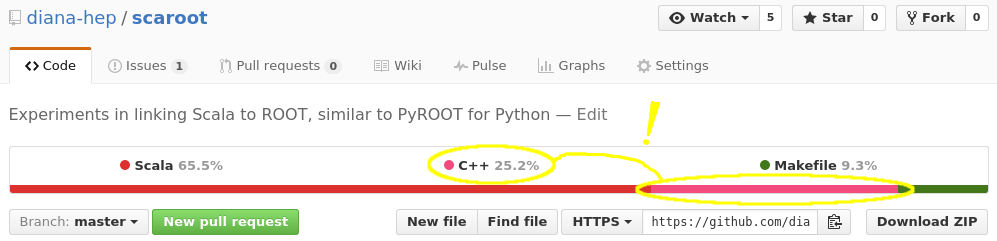
\includegraphics[width=\linewidth]{scaroot_languages.png}

\vspace{0.2 cm}
\begin{itemize}
\item Tested JNI (unsuccessfully) and JNA (successfully).
\begin{itemize}
\item Can open ROOT file and print {\tt ->ls()} from Scala.
\end{itemize}
\item Set up a clean build environment in Maven and Make:
\begin{itemize}
\item {\tt maven clean} deletes {\tt scaroot.so} file.
\item {\tt maven package} runs {\tt make} to build C++ first, then Scala (and any Java, if needed).
\item C-style symbol names ({\tt extern "C"}) in shared object.
\item Assembly puts {\tt scaroot.so} inside {\tt scaroot.jar} for self-sufficienct deployment.
\item User doesn't need to know about {\tt scaroot.so}, but {\tt LD\_LIBRARY\_PATH} must point to ROOT shared objects.
\end{itemize}
\item Namespace: {\tt org.dianahep}, GroupID: {\tt org.diana-hep}.
\end{itemize}
\end{frame}

\end{document}
